\chapter{Local features}

\begin{description}
    \item[Correspondence points] \marginnote{Correspondence points}
        Image points projected from the same 3D point from different views of the scene.

        \begin{example}[Homography]
            Align two images of the same scene to create a larger image.
            Homography requires at least 4 correspondences. 
            To find them, it does the following:
            \begin{itemize}
                \item Independently find salient points in the two images.
                \item Compute a local description of the salient points.
                \item Compare descriptions to find matching points.
            \end{itemize}
        \end{example}


    \item[Local invariant features] \marginnote{Local invariant features}
        Find correspondences in three steps:
        \begin{descriptionlist}
            \item[Detection] \marginnote{Detection}
                Find salient points (keypoints).
            
                The detector should have the following properties:
                \begin{descriptionlist}
                    \item[Repeatability] Find the same keypoints across different images.
                    \item[Saliency] Find keypoints surrounded by informative patterns.
                    \item[Fast] As it must scan the entire image. 
                \end{descriptionlist}
            

            \item[Description] \marginnote{Description}
                Compute a descriptor for each salient point based on its neighborhood.
            
                A descriptor should have the following properties:
                \begin{descriptionlist}
                    \item[Invariant] Robust to as many transformations as possible (i.e. illumination, weather, scaling, viewpoint, \dots).
                    \item[Distinctiveness/robustness trade-off] The description should only capture important information around a keypoint and 
                        ignore irrelevant features or noise.
                    \item[Compactness] The description should be concise.
                \end{descriptionlist}


            \item[Matching] \marginnote{Matching}
                Identify the same descriptor across different images.
        \end{descriptionlist}
\end{description}

\begin{remark}
    Edges are not good interest points as they are locally ambiguous (i.e. pixels are very similar along the direction of the gradient).

    Corners on the other hand are more suited as they have a larger variation along all directions.
\end{remark}


\section{Moravec's corner detector}
\marginnote{Moravec's corner detector}

Given a window $W$ of size $n \times n$,
the cornerness of a pixel $p$ is given by the minimum squared difference between 
the intensity of $W$ centered on $p$ and the intensity of $W$ centered on each of its neighbors:
\[ C(p) = \min_{q \in \mathcal{N}(p)} \Vert W(p) - W(q) \Vert^2 \]

After computing the cornerness of each pixel, one can apply thresholding and then NMS to obtain a matrix where $1$ indicates a corner.

\begin{figure}[H]
    \centering
    \begin{subfigure}{0.3\linewidth}
        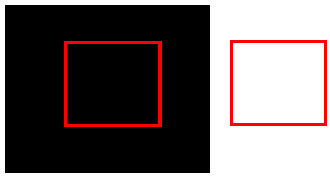
\includegraphics[width=0.9\linewidth]{./img/_corner_detector_example_flat.pdf}
        \caption{Flat region: $C(p)$ is low.}
    \end{subfigure}
    \begin{subfigure}{0.3\linewidth}
        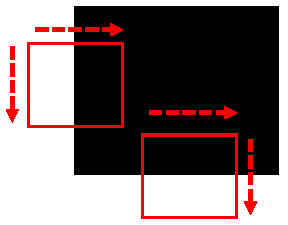
\includegraphics[width=0.8\linewidth]{./img/_corner_detector_example_edge.pdf}
        \caption{Edge: $C(p)$ is low.}
    \end{subfigure}
    \begin{subfigure}{0.3\linewidth}
        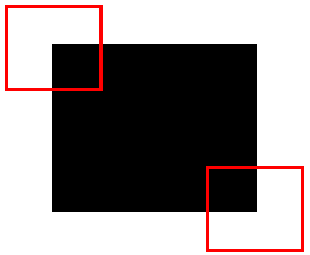
\includegraphics[width=0.8\linewidth]{./img/_corner_detector_example_corner.pdf}
        \caption{Corner: $C(p)$ is high.}
    \end{subfigure}
\end{figure}

\begin{remark}
    Moravec corner detector is isotropic (i.e. independent of the direction).
\end{remark}



\section{Harris' corner detector}

\subsection{Structure matrix}

Harris' corner detector uses an error function formulated as the continuous version of Moravec's detector and 
assumes an infinitesimal shift $(\Delta x, \Delta y)$ of the image:
\[ E(\Delta x, \Delta y) = \sum_{x, y} w(x, y) \big( I(x+\Delta x, y+\Delta y) - I(x, y) \big)^2 \]
where $w(x, y)$ in a window centered on $(x, y)$ and can be seen as a mask with $1$ when the pixel belongs to the window and $0$ otherwise.

By employing the Taylor's series $f(x + \Delta x) = f(x) + f'(x) \Delta x$,
we can expand the intensity difference as:
\[ 
    \begin{split}
        I(x+\Delta x, y+\Delta y) - I(x, y) &\approx \big( I(x, y) + \partial_x I(x, y)\Delta x + \partial_y I(x, y)\Delta y \big) - I(x, y) \\
        &= \partial_x I(x, y)\Delta x + \partial_y I(x, y)\Delta y
    \end{split}
\]

By developing the error function into matrix form, we obtain the following:
\[
    \begin{split}
        E(\Delta x, \Delta y) &= \sum_{x, y} w(x, y) \big( I(x+\Delta x, y+\Delta y) - I(x, y) \big)^2 \\
        &= \sum_{x, y} w(x, y) \big( \partial_x I(x, y)\Delta x + \partial_y I(x, y)\Delta y \big)^2 \\
        &= \sum_{x, y} w(x, y) \big( \partial_x^2 I(x, y)\Delta x^2 + 2 \partial_x I(x, y) \partial_y I(x, y) \Delta x \Delta y + \partial_y^2 I(x, y)\Delta y^2 \big) \\
        &= \sum_{x, y} w(x, y) \left( 
            \begin{bmatrix} \Delta x & \Delta y \end{bmatrix} 
            \begin{bmatrix} 
                \partial_x^2 I(x, y)                    & \partial_x I(x, y) \partial_y I(x, y) \\
                \partial_x I(x, y) \partial_y I(x, y)   & \partial_y^2 I(x, y)
            \end{bmatrix} 
            \begin{bmatrix} \Delta x \\ \Delta y \end{bmatrix} 
        \right) \\
        &= \begin{bmatrix} \Delta x & \Delta y \end{bmatrix} 
            \begin{bmatrix} 
                \sum_{x, y} w(x, y) \partial_x^2 I(x, y)                        & \sum_{x, y} w(x, y) (\partial_x I(x, y) \partial_y I(x, y)) \\
                \sum_{x, y} w(x, y) (\partial_x I(x, y) \partial_y I(x, y))     & \sum_{x, y} w(x, y) \partial_y^2 I(x, y)
            \end{bmatrix} 
            \begin{bmatrix} \Delta x \\ \Delta y \end{bmatrix} \\
        &= \begin{bmatrix} \Delta x & \Delta y \end{bmatrix} 
            \matr{M}
            \begin{bmatrix} \Delta x \\ \Delta y \end{bmatrix} \\
    \end{split}
\]

\begin{description}
    \item[Structure matrix] \marginnote{Structure matrix}
        Matrix $\matr{M}_w$ that encodes the local structure of the image at the pixels within a window $w$.
        \[ \matr{M}_w = \begin{pmatrix} 
            \sum_{x, y} w(x, y) \partial_x^2 I(x, y)                        & \sum_{x, y} w(x, y) (\partial_x I(x, y) \partial_y I(x, y)) \\
            \sum_{x, y} w(x, y) (\partial_x I(x, y) \partial_y I(x, y))     & \sum_{x, y} w(x, y) \partial_y^2 I(x, y)
        \end{pmatrix} \]

        $\matr{M}_w$ is real and symmetric, thus it is diagonalizable through an orthogonal matrix $\matr{R}$:
        \[ \matr{M}_w = \matr{R} \begin{pmatrix} \lambda_1^{(w)} & 0 \\ 0 & \lambda_2^{(w)} \end{pmatrix} \matr{R}^T \]
        $\matr{R}^T$ is the rotation matrix that aligns the image to the eigenvectors of $\matr{M}_w$, 
        while the eigenvalues remain the same for any rotation of the same patch.

        Therefore, the eigenvalues $\lambda_1^{(w)}, \lambda_2^{(w)}$ of $\matr{M}_w$ allow to detect intensity changes along the shift directions:
        \[
            \begin{split}
                E(\Delta x, \Delta y) &= \begin{pmatrix} \Delta x & \Delta y \end{pmatrix} 
                    \begin{pmatrix} \lambda_1^{(w)} & 0 \\ 0 & \lambda_2^{(w)} \end{pmatrix}
                    \begin{pmatrix} \Delta x \\ \Delta y \end{pmatrix} \\
                &= \lambda_1^{(w)} \Delta x^2 + \lambda_2^{(w)} \Delta y^2
            \end{split}
        \]

        \begin{figure}[H]
            \centering
            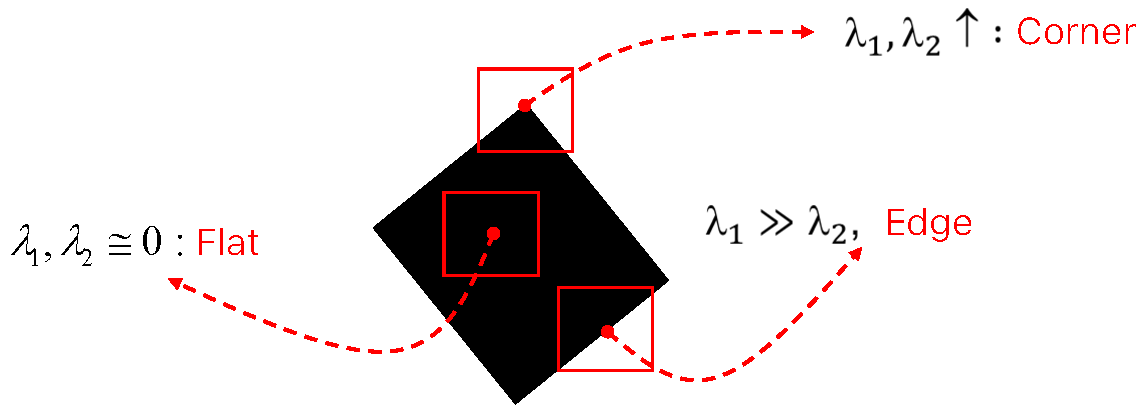
\includegraphics[width=0.6\linewidth]{./img/_harris_rotation.pdf}
            \caption{Eigenvalues relationship at different regions of an image.}
        \end{figure}
\end{description}


\subsection{Algorithm}
\marginnote{Harris' corner detector}

As computing the eigenvalues of $\matr{M}_w$ at each pixel is expensive, a more efficient cornerness function is the following:
\[ 
    \begin{split}
        C(x, y) &= \lambda_1^{(w)}\lambda_2^{(w)} - k(\lambda_1^{(w)} + \lambda_2^{(w)})^2 \\
        &= \det(\matr{M}_{w(x,y)}) - k \cdot \text{trace}(\matr{M}_{w(x,y)})^2 
    \end{split}
\]
where $k$ is a hyperparameter (empirically in $[0.04, 0.06]$).

\begin{figure}[H]
    \centering
    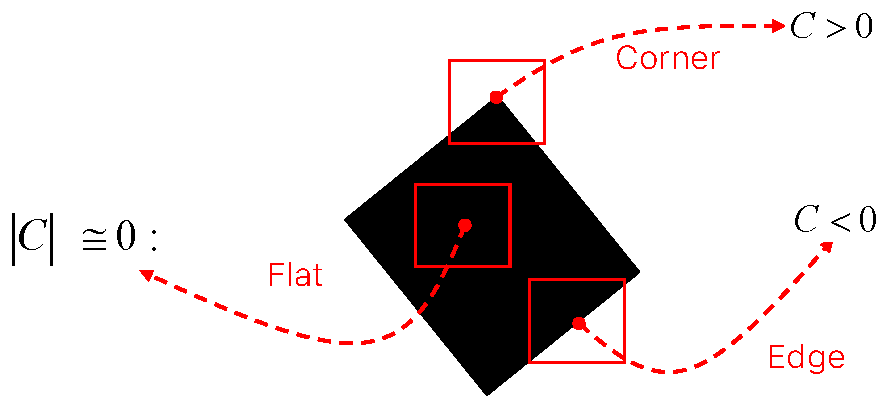
\includegraphics[width=0.5\linewidth]{./img/_harris_efficient.pdf}
    \caption{Cornerness at different regions.}
\end{figure}

After computing the cornerness of each pixel, one can apply thresholding and then NMS.

\begin{remark}
    The window function $w(x, y)$ in the original work follows a Gaussian distribution.
\end{remark}


\subsection{Properties}

Harris' corner detector enjoys the following properties:
\begin{descriptionlist}
    \item[Rotation invariance] 
        The eigenvalues are invariant to a rotation of the image.
    
    \item[No affine intensity change invariance]
        An affine intensity change of a signal consists of a gain factor and the addition of a bias (i.e. $I' = \alpha I + \beta$).
        \begin{description}
            \item[Invariance to bias]
                Harris' detector is invariant to an additive bias ($I' = I + \beta$) as a consequence of the approximate derivative computation:
                \[ 
                    \partial_x I'(i, j) = I'(i, j+1) - I'(i, j) = (I(i, j+1) + \cancel{\beta}) - (I(i, j) + \cancel{\beta})
                \]
            \item[No invariance to gain factor]
                Harris' detector is not invariant to a gain factor ($I' = \alpha I$) as the multiplicative factor is carried in the derivatives.
        \end{description}
        \begin{remark}
            In other words, Harris' detector is not illumination invariant.
        \end{remark}

    \item[No scale invariance]
        Harris' detector is not scale invariant as the use of a fixed window size makes it impossible to recognize the same features when the image is scaled.
\end{descriptionlist}



\section{Multi-scale feature detector}

% \subsection{Scale invariance}

Depending on the scale, an image may exhibit more or less details.
A naive approach consists of using a smaller window size for images with a smaller scale, 
but this is not always able to capture the same features due to the details difference.

\begin{description}
    \item[Scale-space] \marginnote{Scale-space}
        One-parameter family of images obtained by increasingly smoothing the input image.

        \begin{remark}
            When smoothing, small details should disappear and no new structures should be introduced.            
        \end{remark}

        \begin{remark}
            It is possible to use the same window size when working with scale-space images.
        \end{remark}

        \begin{description}
            \item[Gaussian scale-space] \marginnote{Gaussian scale-space}
                Scale-space obtained using Gaussian smoothing:
                \[ L(x, y, \sigma) = I(x, y) * G(x, y, \sigma) \]
                where $\sigma$ is the standard deviation but also the level of scaling.

                \begin{figure}[H]
                    \centering
                    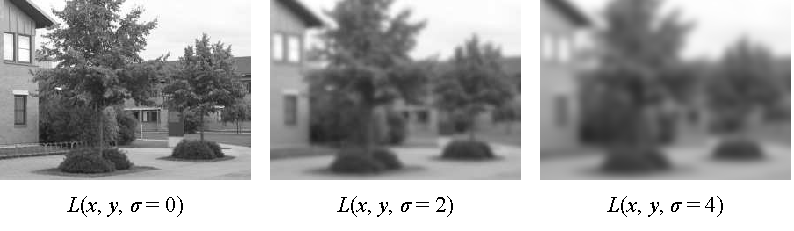
\includegraphics[width=0.8\linewidth]{./img/_scale_space_example.pdf}
                    \caption{Gaussian scale-space example}
                \end{figure}
        \end{description}

    \item[Scale-normalized Laplacian of Gaussian] \marginnote{Scale-normalized Laplacian of Gaussian}
        LOG scaled by a factor of $\sigma^2$:
        \[ F(x, y, \sigma) = \sigma^2 \nabla^2 L(x, y, \sigma) = \sigma^2 (I(x, y) * \nabla^2 G(x, y, \sigma)) \]
        $\sigma^2$ avoids small derivatives when the scaling ($\sigma$) is large.
\end{description}


\subsection{Blob detection}
\marginnote{Scale-normalized LOG blob detection}

Scale-normalized LOG allows the detection of blobs (circles) in an image.

\begin{description}
    \item[Characteristic scale] Scale $\sigma$ that produces a peak in the Laplacian response at a given pixel \cite{slides:scale_normalized_log}.
    
    \item[Algorithm]
        Blob detection using scale-normalized LOG works as follows \cite{slides:scale_normalized_log}:
        \begin{enumerate}
            \item Create a Gaussian scale-space by applying the scale-normalized Laplacian of Gaussian with different values of $\sigma$.
            \item For each pixel, find the characteristic scale and its corresponding Laplacian response across the scale-space (automatic scale selection).
            \item Filter out the pixels whose response is lower than a threshold.
            \item The remaining pixels are the centers of the blobs. 
                It can be shown that the radius is given by $r = \sigma\sqrt{2}$.
        \end{enumerate}
\end{description}


When detecting a peak, there are two cases:
\begin{descriptionlist}
    \item[Maximum] Dark blobs on a light background.
    \item[Minimum] Light blobs on a dark background.
\end{descriptionlist}

\begin{figure}[H]
    \centering
    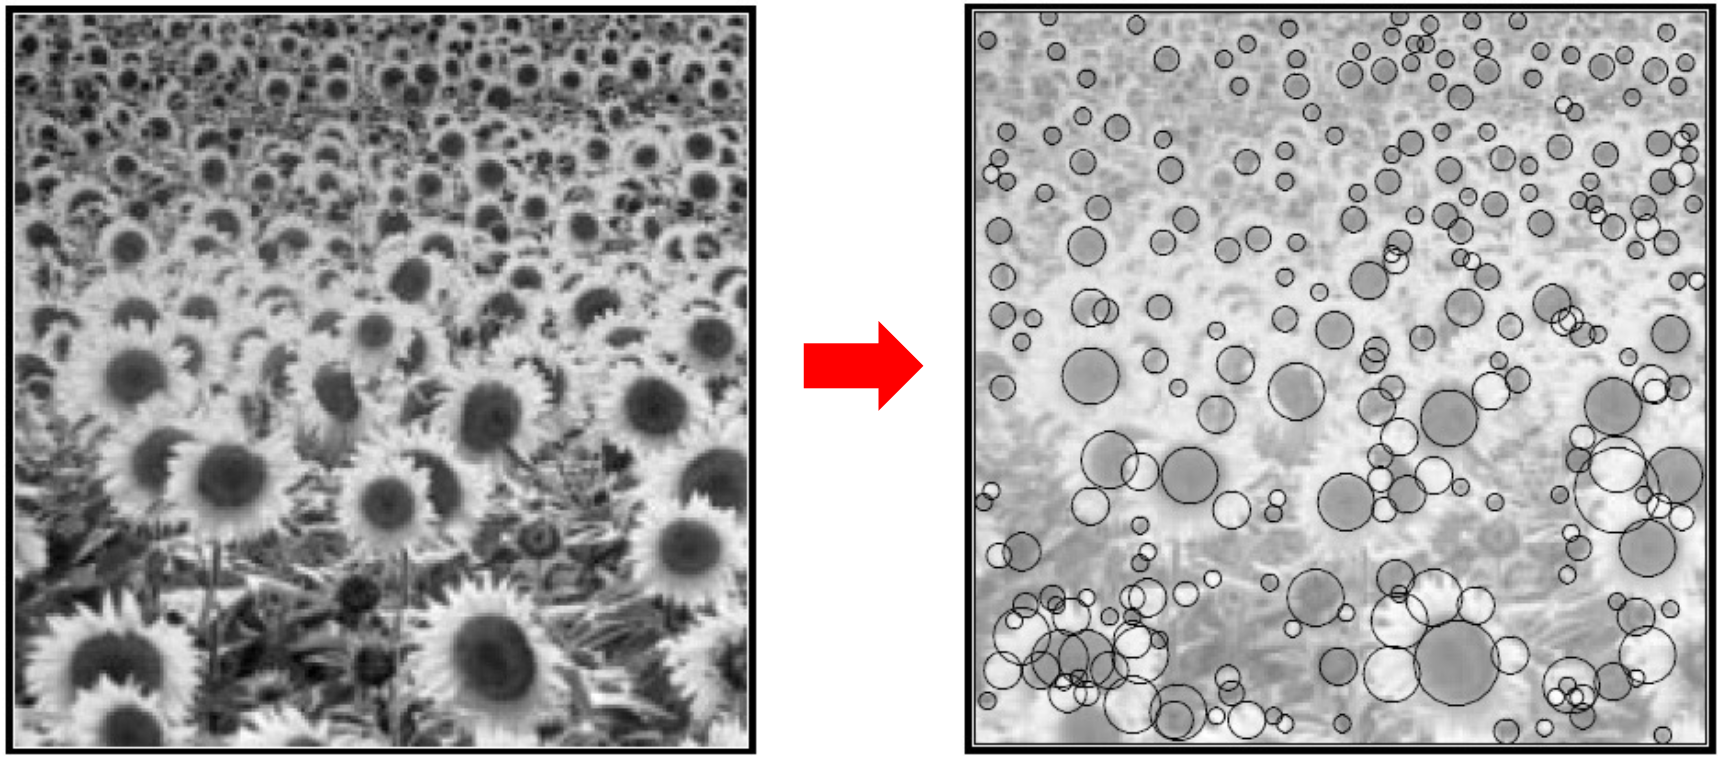
\includegraphics[width=0.6\linewidth]{./img/LOG_blob_detection_example.png}
    \caption{Example of application of the algorithm}
\end{figure}

\begin{remark}
    The intuitive idea of the detection algorithm is the following:
    \begin{itemize}
        \item $F(x, y, \sigma)$ keeps growing for $\sigma$s that capture areas within the blob (i.e. with similar intensity).
        \item The Laplacian reaches its peak when its weights capture the entire blob (virtually it detects an edge).
        \item After the peak, the LOG filter will also capture intensities outside the blob and therefore decrease.
    \end{itemize}
\end{remark}

\begin{remark}
    Using different scales creates the effect of searching in a 3D space.
\end{remark}

\begin{remark}
    It empirically holds that, given two points representing the centers of two blobs,
    the ratio between the two characteristic scales is approximately the ratio between the diameters of the two blobs.
\end{remark}

\begin{figure}[H]
    \centering
    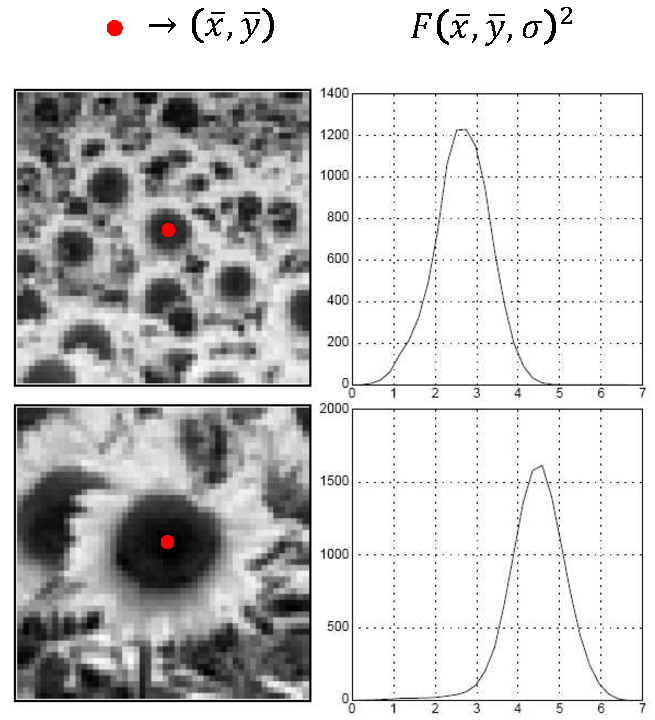
\includegraphics[width=0.4\linewidth]{./img/_scaled_log_blob_diameter.pdf}
    \caption{
        \begin{varwidth}[t]{0.55\linewidth}
            Scale-normalized LOG computed on varying $\sigma$.\\
            Note that, in the second image, the characteristic scale is
            higher as the scale is larger.
        \end{varwidth}
    }
\end{figure}